\documentclass{article}
\usepackage{url}
\usepackage{graphicx}

\title{Master Thesis \\ Recommender Systems Comparison}
\date{27-05-2017}
\author{Vasileios Symeonidis}

\begin{document}
\maketitle
\newpage
\tableofcontents
\pagenumbering{gobble}
\newpage
\pagenumbering{roman}

\section{Intro}

\section{Collaborative filtering}
\subsection{Content based}
\subsection{Latent Factors}

\begin{figure}
\centering
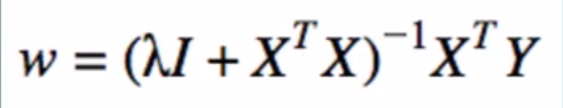
\includegraphics[width=0.7\linewidth]{/home/d4md1n/Downloads/equation01}
\caption{}
\label{fig:equation01}
\end{figure}

\section{Our Experiment}
\subsection{Infrastructure}
\subsubsection{Apache Spark}
\subsection{Dataset}
\subsection{Metrics}
\subsubsection{Mean Absolute Error}
\subsubsection{Execution Time}
\cite{ApacheSpark:1}
\cite{RecommenderSystems:2}
\cite{MovieLens:3}

\section{Results}
\section{Conclusion}
\section{references}

\appendix
\part{test}
\section{Appendix relevant code}
\subsection{Appendix A.a: User Based Collaborative Filtering	8}
\subsection{Appendix A.b: Product Based Collaborative Filtering	8}
\subsection{Appendix A.c: Latent Factors}
\section{\\Title of Appendix A}
% the \\ insures the section title is centered below the phrase: AppendixA

Text of Appendix A is Here

\section{\\Title of Appendix B}
% the \\ insures the section title is centered below the phrase: Appendix B

Text of Appendix B is Here

\section{apendixB Metrics}
\section{apendixC List of Figures}
\listoffigures


\section{apendixC List of Tables}
\listoftables
\newpage
\bibliography{thesis}
\bibliographystyle{ieeetr}
%\footnote{}
%\cite{DUMMY:1}
%https://www.sharelatex.com/learn/Lists_of_tables_and_figures
\end{document}
